\documentclass[border=10pt]{standalone} 
\usepackage[utf8]{inputenc}
\usepackage{nacal}
\usepackage{pgfplots}
\usepackage{tikz-3dplot}
\usepackage{tikz} 
\usetikzlibrary{matrix,decorations.pathreplacing}
\usetikzlibrary{calc,angles,positioning,intersections,quotes,decorations.markings}
\usepackage{tkz-euclide}

\pgfplotsset{width=10cm,height=6cm}

\begin{document}
  \def\Rojo{red!50!black}
  \def\RojoOscuro{red!20!black}
  \def\RojoClaro{red!90!black}
  \def\Verde{green!50!black}
  \def\VerdeOscuro{green!30!black}
  \def\VerdeClaro{green!50!gray}
  \def\Azul{blue!50!black}
  \def\AzulOscuro{blue!35!black}
  \def\AzulClaro{blue!60!gray}

  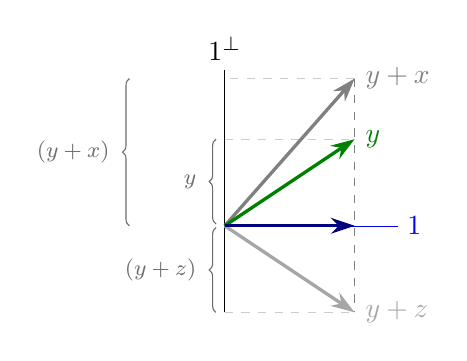
\begin{tikzpicture}[scale=1.1]
    % vértices del triángulo
    \coordinate (v1) at (0,0);
    \coordinate (v2) at (2,0); % punta eje horizontal
    \coordinate (v3) at (1.5,1.7);
    
    \coordinate (v4) at (1.5,0);  
    
    \coordinate (v6) at (0,1.7); % vector e
    \coordinate (v7) at (0,1.8); % punta eje vertical

    %\coordinate (v8) at (1.5,1.7);
    \coordinate (v9) at (1.5,2.5);  
    \coordinate (v10) at (1.5,3);  
    \coordinate (v11) at (1.5,1);  
    \coordinate (v12) at (1.5,-1);  
    \coordinate (v13) at (0,-1);  
    \coordinate (v14) at (0,1);  

    % division del triangulo
    \draw[-,gray,dashed,very thin]  (v3) -- (v12);
    \draw[-,gray!40,dashed,very thin]  (v3) -- (v6);
    \draw[-,gray!40,dashed,very thin]  (v14) -- (v11);
    \draw[-,gray!40,dashed,very thin]  (v13) -- (v12);
    
    \draw[color=blue!95!black,very thin]  (v1) -- (v2) node [right]  {$\Span{\Vect{1}}$};
    \draw[very thin]  (v13) -- (v7) node [above]  {$\Span{\Vect{1}}^\perp$};
    \draw[-{Stealth[length=3mm, width=2mm]},very thick, gray] (v1) -- (v3) node [anchor=west]  {$\Vect{y}+\Vect{x}$};
    
    \draw[-{Stealth[length=3mm, width=2mm]},very thick,green!50!black] (v1) -- (v11) node [anchor= west]  {$\Vect{y}$};
    \draw[-{Stealth[length=3mm, width=2mm]},very thick, gray!70] (v1) -- (v12) node [anchor=west]  {$\Vect{y}+\Vect{z}$};

    \draw[-{Stealth[length=3mm, width=2mm]},very thick,blue!50!black] (v1) -- (v4); % node [below,yshift=-1mm]  {$\Vect{\media{y}}$}; ,gray!70!blue!80

    \draw[decorate, decoration={brace},gray!85!black] (-0.1,0.02) -- (-0.1,1) node [midway, anchor=east, xshift=-1mm, outer sep=1pt,font=\footnotesize]{$\dt{\Vect{y}}$};
    \draw[decorate, decoration={brace},gray!85!black] (-0.1,-1) -- (-0.1,-0.02) node [midway, anchor=east, xshift=-1mm, outer sep=1pt,font=\footnotesize]{$\dt{(\Vect{y}+\Vect{z})}$};
    \draw[decorate, decoration={brace},gray!85!black] (-1.1,0) -- (-1.1,1.7) node [midway, anchor=east, xshift=-1mm, outer sep=1pt,font=\footnotesize]{$\dt{(\Vect{y}+\Vect{x})}$};
    
  \end{tikzpicture} 
\end{document}
